\subsection{課題説明}
3種類の連続関数$y=x^2$、$z=x^2+y^2$、$y=-x \times sin(x)$について、
最急降下法の適用を通して探索挙動を観察した。
以下ではまず共通部分である最急降下法の探索手続きについて、
フローチャートを用いて解説する。
その後、3種類の関数毎にプログラムの変更箇所、
観察意図観察方法、観察結果、考察について説明する。

\subsubsection{探索の手続き(共通部分)}
今回の探索において適用される最急降下法は次のように値を更新していく
\[x_{next} = x -α*f'(x)\]
学習係数αは 0 より大きい実数とし、この値の更新を繰り返すことにより
最適解(最小値)を探索することができる.

\subsubsection{フローチャート(共通部分)}
(手続きとフローチャートはまとめて一つの節にしても構いません)
	\begin{figure}[h!]
  		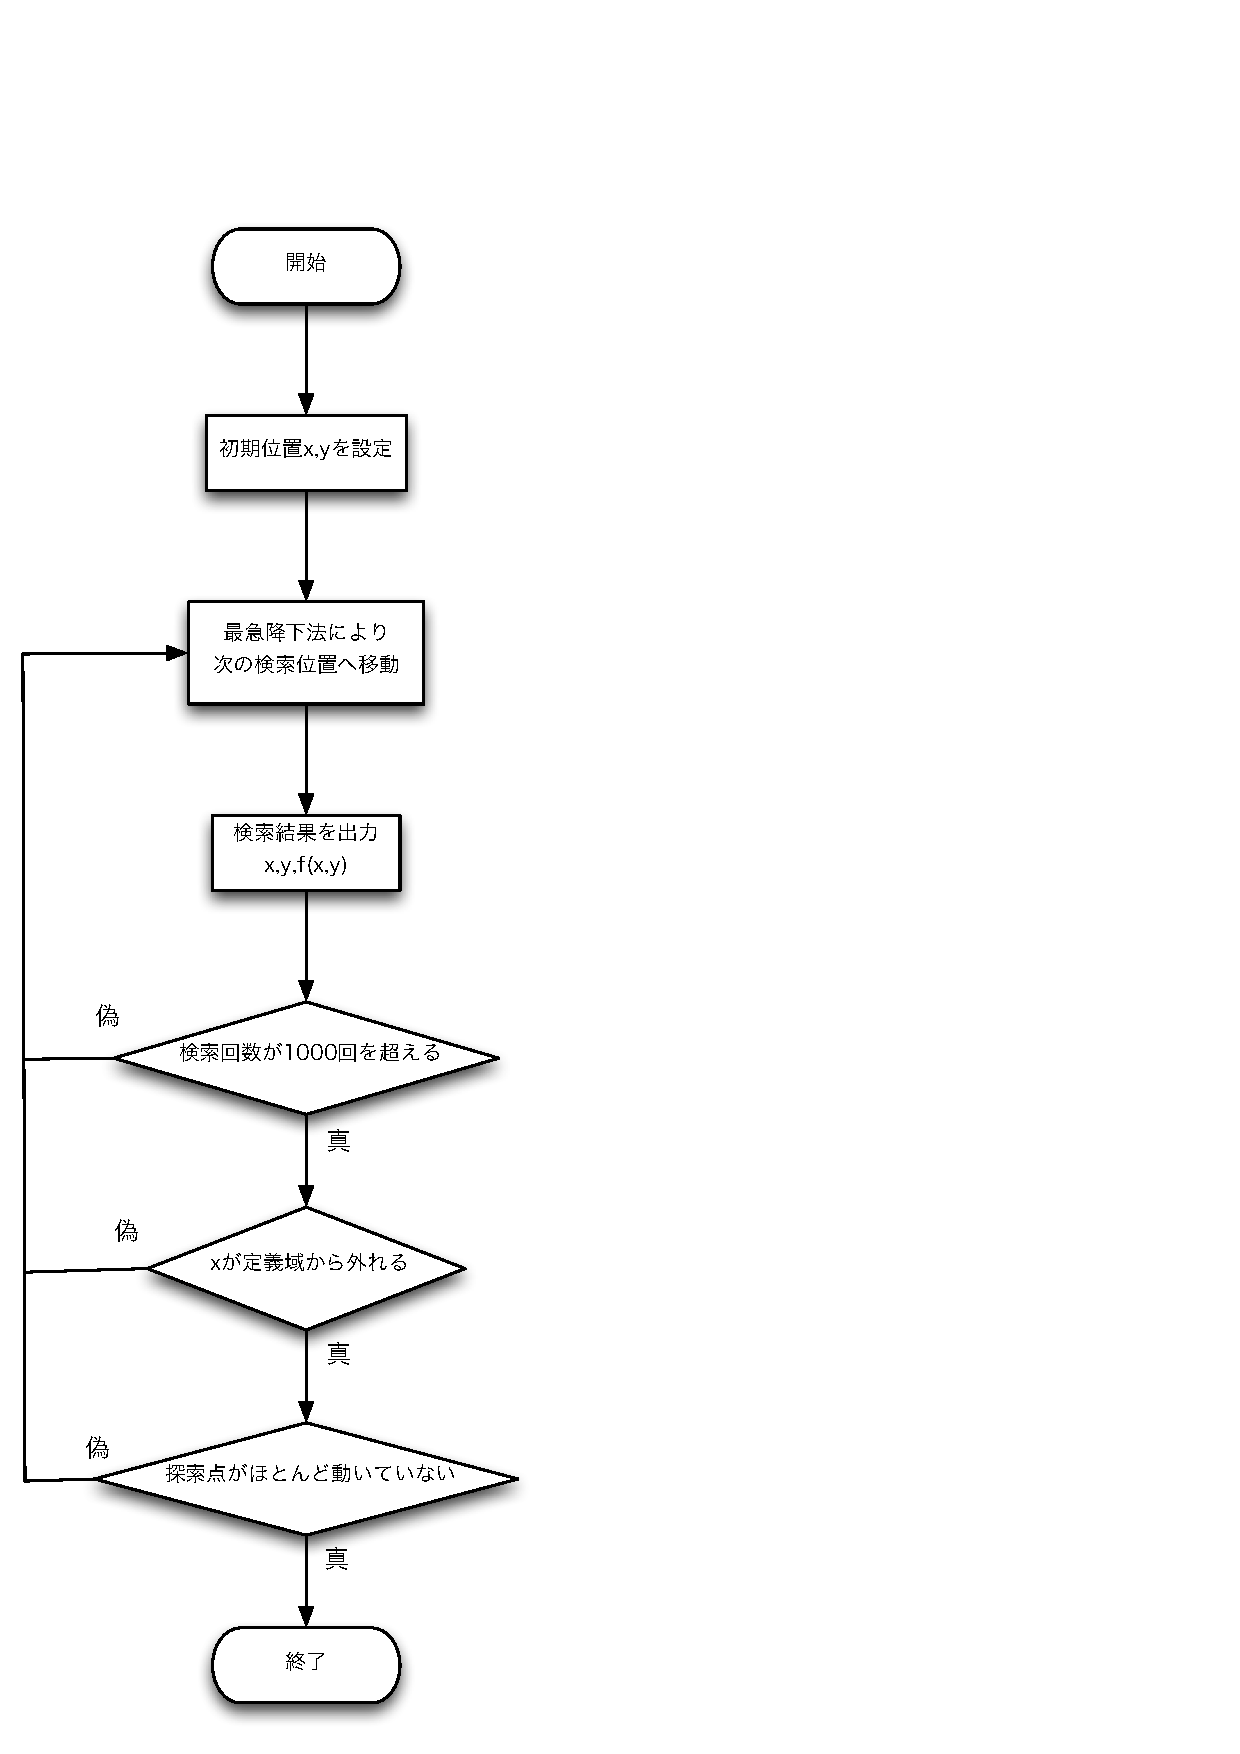
\includegraphics[clip,width=5.0cm]{flowchart.pdf}
	\end{figure}

